
\documentclass[11pt]{amsart}
\usepackage[left=2cm,top=2cm,right=2cm,bottom=2cm,nohead,foot=2cm]{geometry}
\geometry{letterpaper}
\usepackage[parfill]{parskip}
\usepackage{graphicx}
\usepackage{amssymb}
\usepackage{amsmath}
\usepackage{float}
\usepackage{epstopdf}
\usepackage{moreverb}
\usepackage{multicol}
\usepackage{comment}
\usepackage{wrapfig}
\DeclareGraphicsRule{.tif}{png}{.png}{`convert #1 `dirname #1`/`basename #1 .tif`.png}
\DeclareGraphicsExtensions{.pdf,.png,.jpg}

%creating solution environment
\specialcomment{sol}{\textbf{Solution: }}{}
%this command toggles the solutions
%\excludecomment{sol} %comment this to SHOW solutions

%For the lazy:
\newcommand{\ds}{\displaystyle}
\newcommand{\be}{\begin{enumerate}}
\newcommand{\ee}{\end{enumerate}}
\newcommand{\mrm}{\mathrm}
\newcommand{\bee}{\begin{eqnarray*}}
\newcommand{\eee}{\end{eqnarray*}}
\newcommand{\dds}[2]{\frac{\mathrm{d}#2}{\mathrm{d}#1}} %(d1 BY d2)
\newcommand{\ddb}[2]{\frac{\mathrm{d}}{\mathrm{d}#1}\left[ #2\right]}
%(d by d1 OF 2)

\begin{document}

\begin{minipage}{0.5\textwidth}
		\noindent {\bf CSCI 2824 -- Spring 2020}
\end{minipage}\hfill
\begin{minipage}{0.5\textwidth}
		\noindent \hfill {\bf Homework 6}
\end{minipage}
\noindent This assignment is due on Friday, February 28 to Gradescope by 11:59pm.  You are expected to write up your solutions neatly and \textbf{use the coverpage}.  Remember that you are encouraged to discuss problems with your classmates, but you must work and write your solutions on your own. 

{\bf Important}: On the {\bf official CSCI 2824 cover page} of your assignment clearly write your full name, the lecture section you belong to (001 or 002), and your student ID number.  You may \textbf{neatly} type your solutions for +2 extra credit on the assignment. You will lose \textit{all} 5 style/neatness points if you fail to use the official cover page.

\vspace{5mm}
\be
%==============================================================================
% Set Properties
%==============================================================================
\item In an in-class example, we observed anecdotally that for non-empty sets $P, Q,$ and $R$, the following holds: $$(P \cap Q) \times R = \left( P \times R\right) \cap \left( Q \times R\right)  $$
	\be
		\item Prove that $(P \cap Q) \times R = \left( P \times R\right) \cap \left( Q \times R\right)  $ holds by showing that each side of this equation is a subset of the other side of the equation.
		\item Prove that that $(P \cap Q) \times R = \left( P \times R\right) \cap \left( Q \times R\right)  $ holds using \textbf{set builder} notation and using set identities.
	\ee

	\begin{sol}
	\be
		\item Let $Z \in (P \cap Q) \times R$\\
		$z = (x,y), \; x \in P \cap Q$ and $y \in R$\\
		$(x \in P$ and $x \in Q)$ and $y \in R$\\
		$(x \in P$ and $y \in R)$ and $(x \in Q$ and $y \in R)$\\
		$(x,y) \in P \times R$ and $(x,y) \in Q \times R$\\
		$(x,y) \in (P \times R) \cap (Q \times R)$\\
		$z \in (P \times R) \cap (Q \times R)$\\
		$\therefore (P \cap Q) \times R \subseteq (P \times R) \cap (Q \times R)$\\
		\\
		Now, $z \in (P \times R) \cap (Q \times R)$\\
		$z \in P \times R$ and $z \in Q \times R$\\
		$(x,y) \in P \times R$ and $(x,y) \in Q \times R$\\
		As before, $(x \in P$ and $x \in Q)$ and $y \in R$\\
		$x \in P \cap Q$ and $y \in R$\\
		$(x,y) \in (P \cap Q) \times R$\\
		$z \in (P \cap Q) \times R$\\
		$\therefore (P \times R) \cap (Q \times R) \subseteq (P \cap Q) \times R$\\
		\\
		$\therefore (P \cap Q) \times R = (P \times R) \cap (Q \times R)$

		\item
		\begin{math}
			(P \cap Q) \times R\\
			= \{ (x,y): x \in P \cap Q, \; y \in R \}\\
			= \{ (x,y): x \in P \text{and} x \in Q, \; y \in R \}\\
			= \{ (x,y): x \in P, \; y \in R \} \text{ and } \{ (x,y): x \in Q, \; y \in R \}\\
			= \{ (x,y): x \in P, \; y \in R \} \cap \{ (x,y): x \in Q, \; y \in R \}\\
			= (P \times R) \cap (Q \times R)
		\end{math}
	\ee
	\end{sol}

%==============================================================================
% Recurrences
%==============================================================================
\item Complete the following recurrence exercises:
	\be
		\item Find a closed form of the recurrence given by $a_n=7\cdot  a_{n-1}-5;\, a_0=4$
		\item Find a closed form of the recurrence given by $a_n=(n+1)^2\cdot  a_{n-1};\, a_0=1$
		\item Consider the recurrence $a_n=a_{n-1}+2a_{n-2}+2n-9.$
			\be
				\item Show that this recurrence is solved by $a_n=2-n$.
				\item Show that this recurrence is solved by $a_n=2-n+b\cdot2^n$ for any real $b$.
			\ee
	\ee

	\begin{sol}
	\be
		\item $a_n - 7a_{n-1} = -5$\\
		Express $a_n - 7a_{n-1} = -5$ for all $n = n, (n-1), \textellipsis ,1$\\
		$a_n - 7a_{n-1} = -5\\
		7a_{n-1} - 7^2a_{n-2} = -5 \cdot 7\\
		7^2a_{n-2} - 7^3 a_{n-3} = -5 \cdot 7^2\\
		\textellipsis\\
		\textellipsis\\
		7^{n-1}a_1 - 7^na_0 = -5 \cdot 7^{n-1}\\
		a_n - 7^na_0 = -5 - 5 \cdot 7 - 5 \cdot 7^2 - \textellipsis - 5 \cdot 7^{n-1}\\
		a_0 = 4\\
		\therefore a_n - 4 \cdot 7^n = -5(1 + 7 + 7^2 + \textellipsis + 7^{n-1})\\
		a_n - 4 \cdot 7^n = -5(\frac{1(7^n - 1)}{7 - 1})\\
		a_n = 4 \cdot 7^n - \frac{5(7^n - 1)}{6}\\
		a_n = \frac{24 \cdot 7^n - 5 \cdot 7^n + 5}{6}\\
		a_n = \frac{19 \cdot 7^n + 5}{6}$
		\item $a_n = (n + 1)^2 \cdot n^2 \cdot a_{n-2}$\\
		$= (n + 1)^2 \cdot n^2 \cdot (n - 1)^2 \cdot a_{n-3}$\\
		$= (n + 1)^2 \cdot n^2 \cdot (n - 1)^2 \ldots 2^2 \cdot a_0$\\
		$a_n = (n + 1)^2$
		\item
		\be
			\item $a_n = 2 - n = 2 - (n - 1) + 2 (2 - (n - 2)) + 2n - 9$\\
			$2 - n = 3 - n + 8 - 2n + 2n - 9$\\
			$2 - n = 2 - n$
			\item $a_n = 2 - n + b \cdot 2^n = 2 - (n - 1) + b \cdot 2^{n-1} + 2(2 - (n - 2) + b \cdot 2^{n-2}) + 2n - 9$\\
			$= 2 - n + b \cdot n^{n-1} + 2b \cdot 2^{n-2}$\\
			$= 2 - n + 2b \cdot 2^{n-1}$\\
			$= 2 - n + b \cdot 2^n$
		\ee
	\ee
	\end{sol}

%==============================================================================
% Functions: 1-1, Onto, etc.
%==============================================================================
\item Consider the function $f: \mathbb{Z} \times \mathbb{Z} \rightarrow \mathbb{Z}$ given by $f(n,m)=\frac{n^3}{|m|+1}$
	\be
		\item Write in logical predicate notation - using quantifiers for $n$, $m$, etc. as appropriate - the logical equivalent of the function $f$ being onto.
		\item Determine whether or not $f$ is one-to-one.
		\item Determine whether or not $f$ is onto.
	\ee
	\begin{sol}
		\be
			\item $f$ is onto iff:\\
			$\forall y \in \mathbb{Z} \; \exists (n,m) \in \mathbb{Z} \times \mathbb{Z}$ such that $f(n,m) = y$
			\item $f(0,1) = 0$ and $f(0,2) = 0$\\
			$f(0,1) = f(0,2)$ but $(0,1) \ne (0,2)$\\
			$f$ \textbf{IS NOT} one-to-one
			\item define $y \in \mathbb{Z}$ then observe:\\
			$f(y,y) = \frac{y^3}{|y^2 - 1| + 1} = y$\\
			$\therefore \forall y \in \mathbb{Z} \; \exists (n,m) \in \mathbb{Z} \times \mathbb{Z}$ such that $f(n,m) = y$\\
			$\therefore f$ \textbf{IS} onto
		\ee
	\end{sol}

%==============================================================================
% Onto and 1-1, as sets
%==============================================================================
\item Define the set $C=$ the set of all Spring 2020 CSCI2824 students.
\be
	\item Define in words a function $f: C \rightarrow \mathbb{Z}$.  Is the function function one-to-one and/or onto? Be sure that $f$ is actually a function, and feel free to be creative!
	\item Again define the set $C=$ the set of all Spring 2020 CSCI2824 students.  Define in words another function $g: C \rightarrow \mathbb{Z}$, but ensure that $g$ is definitely one-to-one. 
\ee

\begin{sol}
	\be
		\item def $C=$ the set of all CSCI2824 students as stated above\\
		def $f: C \rightarrow \mathbb{Z}$ as student $\rightarrow$ their height\\
		This is a function, however it \textbf{WILL NOT BE ONTO} as the range is finite and the codomain is infinite.\\
		Given the fact two or more people in the class are most likely the same height, this function \textbf{WILL NOT BE ONE-TO-ONE}.
		\item def $C=$ the set of all CSCI2824 students as stated above\\
		def $f: C \rightarrow \mathbb{Z}$ as student $\rightarrow$ their Social Security Number\\
		This is a function, and each student is mapped to their individual and unique SSN, meaning this function \textbf{WILL BE ONE-TO-ONE}
	\ee
\end{sol}

%==============================================================================
% Alg complexity intro
%==============================================================================	
\item The given code attempts to answer the popular debate: ``which Jedi wins in a duel?"  \\
	The code:\\
	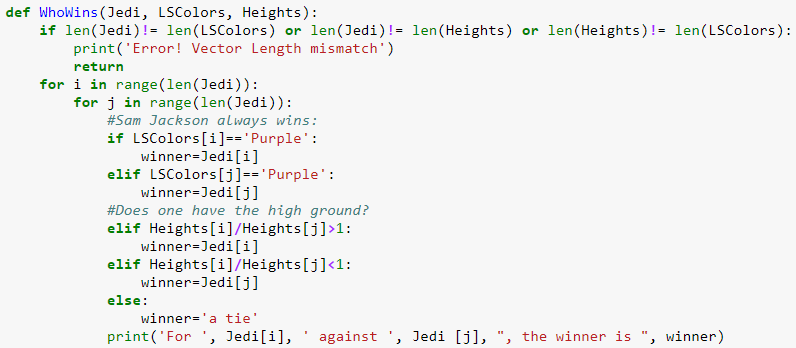
\includegraphics[width=.6\textwidth]{JediCode}\\
	\be
		\item[i)] Makes sure the inputs - Jedi names, lightsaber colors, and current topographic information - are the same sizes.
		\item[ii)] Pairs up Jedi within a couple of for loops
		\item[iii)] Checks if Jedi \#1 is Mace or if Jedi \#2 is Mace. He always wins in these debates.
		\item[iv)] Checks which Jedi is currently at the highest elevation.  After all, the high ground wins!
	\ee
	You, aspiring Jedi enthusiast, must answer:
	\be
		\item What is the \textbf{algorithmic complexity} of this code?  In other words, exactly how comparisons are checked if $n$ Jedi are input correctly?  You may assume that \textit{each} part of the \textbf{if, elif, else} statement does in fact generate a comparison regardless of input, as this is a ``worst-case" analysis.
		\item What are some redundancies of this code?  Could it be done in less comparisons?
		\item (Not for points): In your opinion, what should actually have been used to determine the winners?
	\ee
	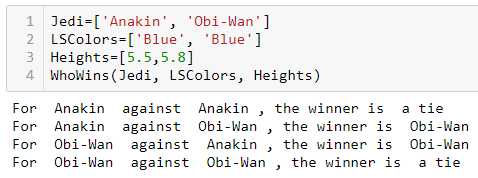
\includegraphics[width=.6\textwidth]{JediOutput}\\
\begin{sol}
	\be
		\item Assuming the 3 lists are inputted correctly, the code would perform $5n^2$ comparisions in total, as there are 5 comparisons with in a nested for loop iterating $n$ times.
		\item Defining the 'winner' variable as 'a tie' at the beginning saves one comparison, then you simply reassign it if either of the Jedi do win. This would take the comparisons in each loop down to 4. The code would end up looking something like:\\
		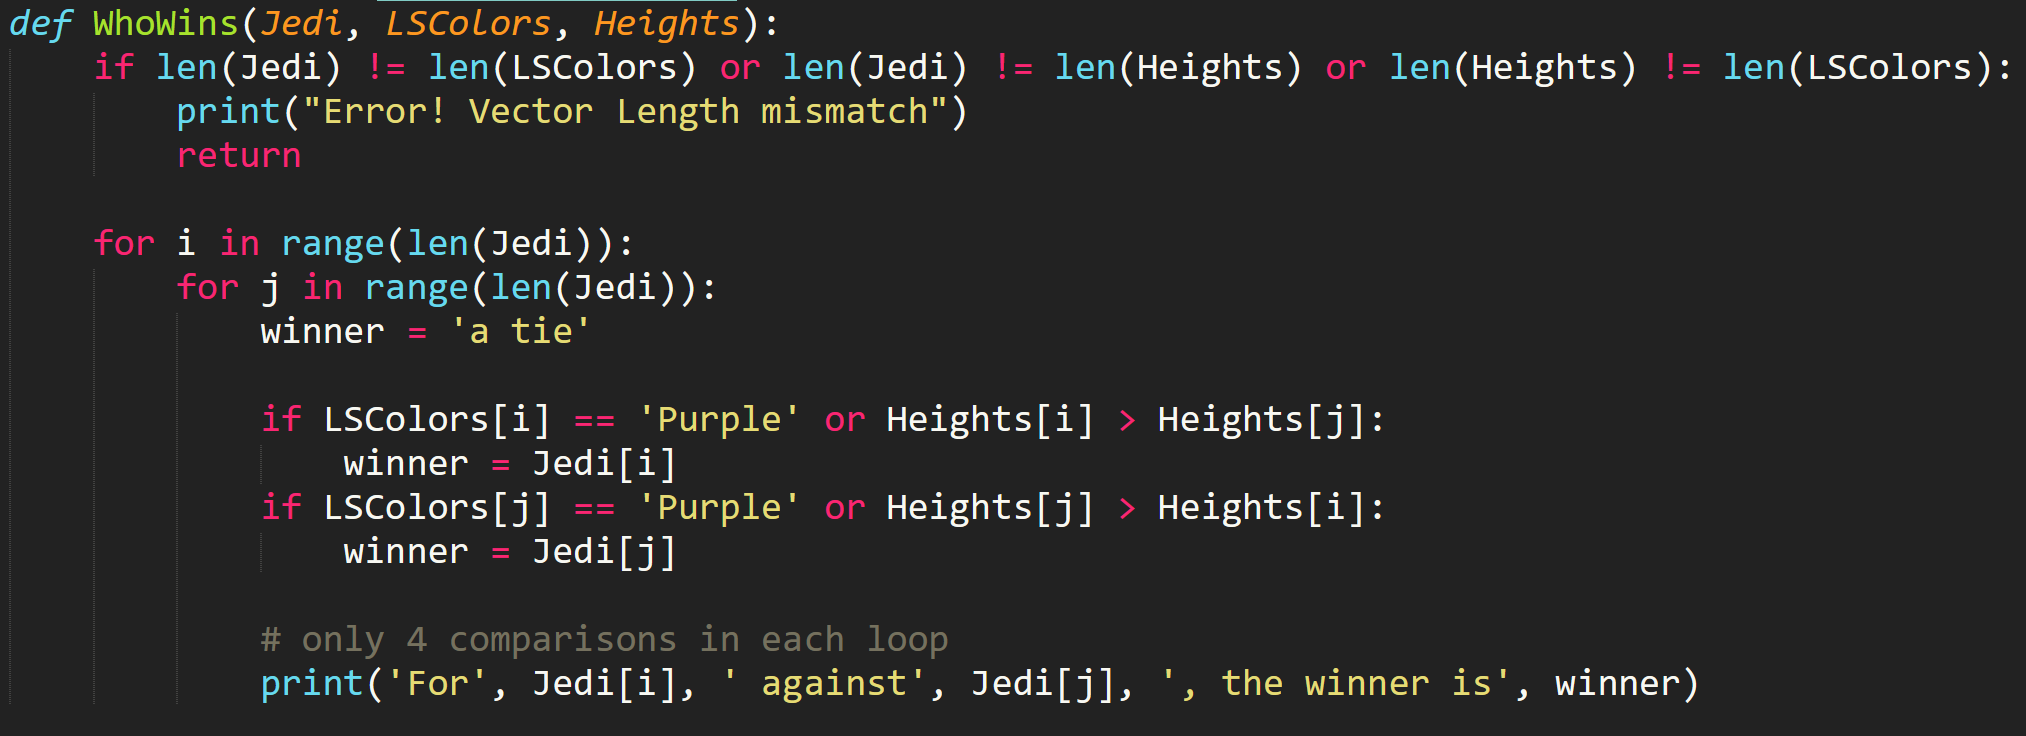
\includegraphics[width=.6\textwidth]{newCode}
		\item I agree with taking lightsaber color into account, but everyone knows that the coolest lightsaber color is yellow, therefore that should be the winning color. Instead of height, the rank of the Jedi in question should determine who would win in every other case, with the highest rank Jedi winning and a tie resulting if two Jedi are the same rank.
	\ee
\end{sol}

\ee

\end{document}